\subsection{Taxi Manager}\label{comp:taxiManager}
\subsubsection{Internal Components}
The Taxi Manager is responsible for the communication with taxi drivers, and for the management of their life cycle. Internally it is composed of the following components each with a precise job:
\begin{itemize}
	\item \textit{TaxiLifeCycleManager}: it manages the life cycle of taxi drivers. In order to do so it exposes an interface for setting the availability status, and for updating the location. It stores all the informations related to taxi drivers through the DataAccess. If a taxi driver sets himself as Available, the component will call the add method of the QueueManager. Oppositely if the taxi driver sets himself as NotAvailable, it will call the remove method. When a taxi driver updates his location, the component computes the zone through the GeographicEngine; if it notices that the zone has changed, it calls the changeZone method of the Taxi Manager. It also exposes an internal interface to the TaxiDispatcher, which is meant to be used to set the status of a taxi driver as Busy once he accepts a request.
	\item \textit{TaxiDispatcher}: it exposes the interface for providing a taxi driver for a location. Once it has been called he first compute the corresponding zone for the location provided, then it starts a loop where it calls the QueueManager for getting a taxi. If there are no taxi available in that zone he returns a negative message, otherwise it forwards the request to the taxi driver it got as a response. If the taxi driver accepts, it set his status as Busy through the TaxiLifeCycleManager and return him to the caller. If the taxi driver does not accept, it starts the loop again.
\end{itemize}
\begin{figure}[H]
	\centering
	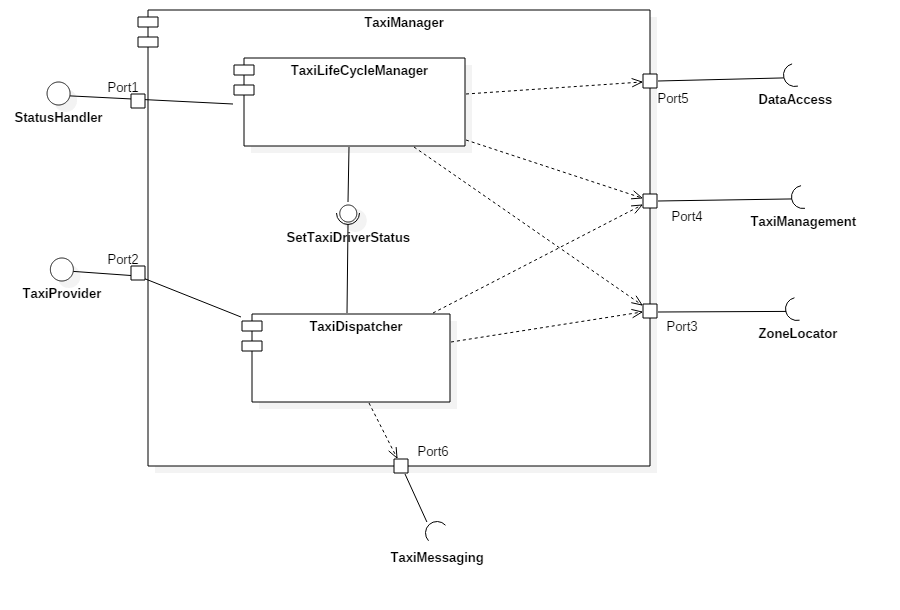
\includegraphics[scale=0.5]{../"Analysis Documents"/components/taxiManager}
	\label{fig:taximanager}
	\caption{Taxi Manager internal structure}
\end{figure}
\subsubsection{Provided interfaces}
\begin{table}[H]
	\begin{longtable}{| p{0.3\textwidth} | p{0.3\textwidth} | p{0.4\textwidth} |}
		\hline
		\textbf{Provided Interface} & \textbf{Dedicated user} & \textbf{Description} \\ \hline
		StatusHandler & The Taxi driver's mobile application & Allows the taxi driver to set himself as 'Available' and 'Not Available'. Plus, it is used from the application to communicate the current location \\ \hline
		TaxiProvider & Ride Manager component & Given a location, it provides a taxi (if the correspondent queue is not empty and one taxi accepts) \\ \hline
	\end{longtable}
	\caption{Taxi manager: provided interfaces}
	\label{tab:taximanager:providedInterfaces}
\end{table}
\subsubsection{Required interfaces}
\begin{table}[H]
	\begin{longtable}{| l | p{.80\textwidth} |}
		\hline
		\textbf{Required Interface} & \textbf{Description and usage} \\ \hline
		ZoneLocator & Retrieves the correspondent zone of a location \\ \hline
		DataAccess & Save the information of the taxi driver status \\ \hline
		TaxiManagement & It communicates to the data structure containing the taxi drivers, whether to add, remove or retrieve them. \\ \hline
	\end{longtable}
	\caption{Taxi manager: required interfaces}
	\label{tab:taximanager:requiredInterfaces}
\end{table}
